\chapter{Proposed Solution}

	%https://martinfowler.com/articles/microservices.html
	%
	This chapter contains the details of the implementation of the solution as well as a description of the components involved in the application.
	The high level architecture of the solution was designed with the separation of responsibilities in mind. It's divided in three main components, the front-end application, the server web \gls{api} and the database.
	
	The database was needed to store the user data and reminders. 
	Since the data would be structured it was decided to use a relational database.
	There were two databases considered for this: PostgreSQL and MySQL. Although MySQL has faster read speeds \cite{db-speed} which would advantageous for the task service, PostgreSQL was chosen since it was already known and easier to integrate with NodeJS.
	
	\section{database}
	
	
	\section{title}
	
	\begin{figure}[h!]
		\centering
		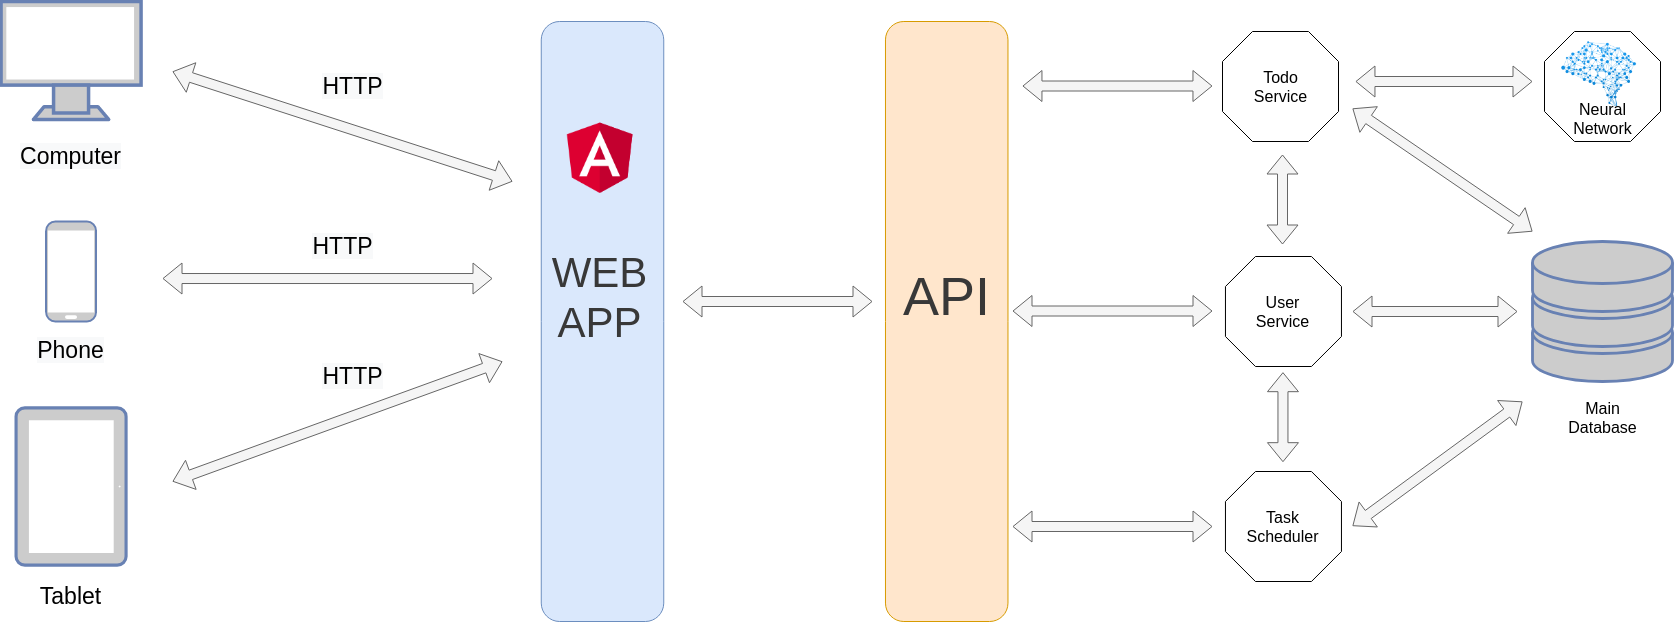
\includegraphics[width=\linewidth]{./images/abstract_architecture}
		\caption{High level architecture}
	\end{figure}
	
	The architecture for the web \gls{api} was thoroughly researched and studied. At first this project was gonna use a monolithic architecture \cite{monolith} where the whole \gls{api} would be implement on a single server as seen in the image below.

	\begin{figure}[h!]
		\centering
		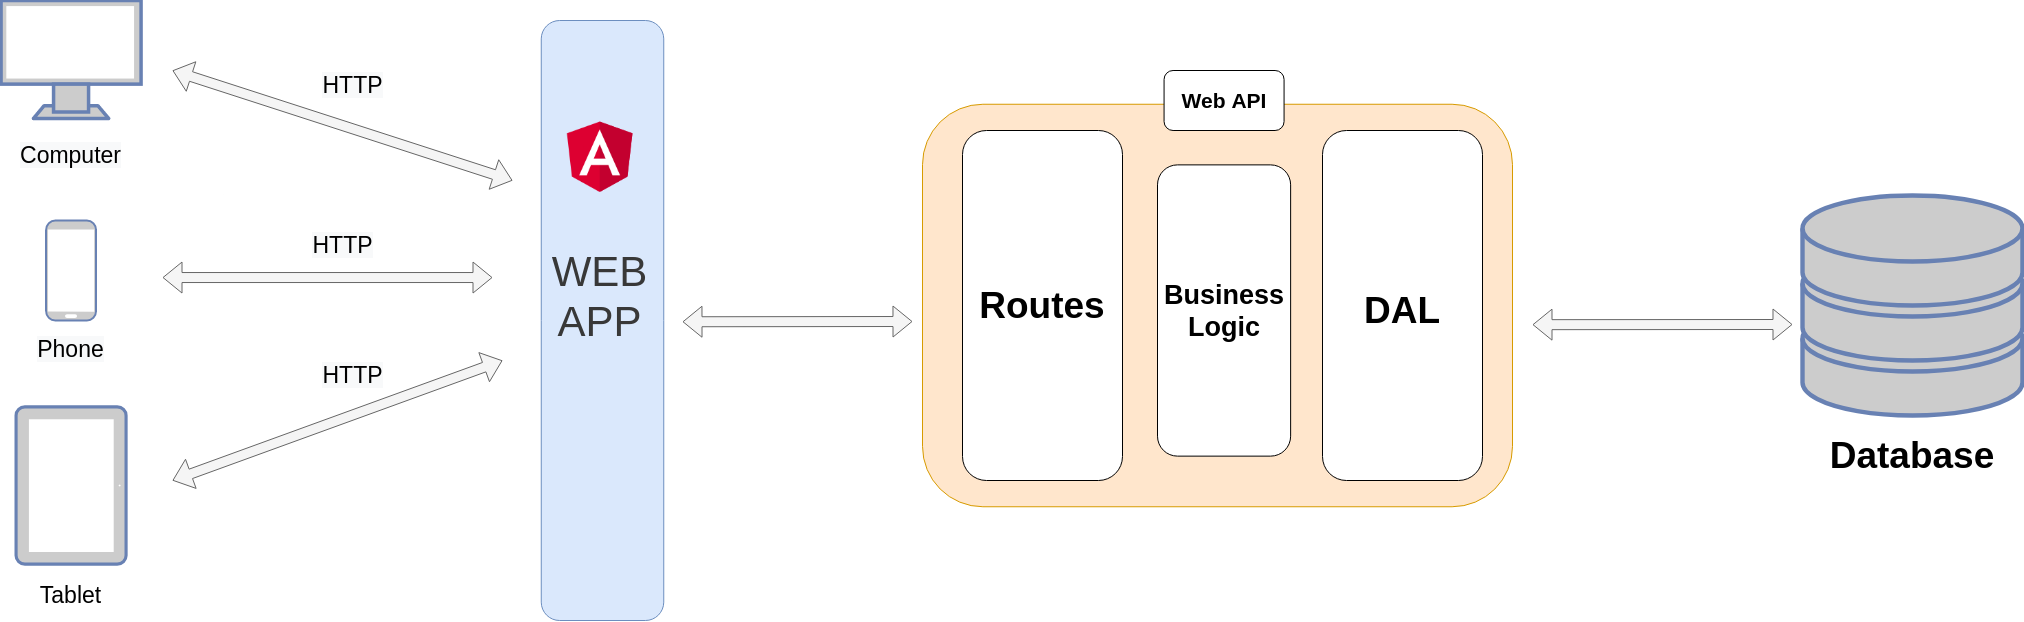
\includegraphics[width=\linewidth]{./images/monolithic_abstract_architecture}
		\caption{Abstract monolithic architecture}
	\end{figure}
	
	This was later changed due to the fact that it wasn't as easily scalable \cite{scale}. After this it was decided that the \gls{api} would be implemented using a micro-service\cite{microservice} architecture. This allows for a more select scalability. When needed, more instances of the same services can be launched and improve overall performance.
	
	There are three different services:
	\begin{enumerate}
		\item User
		\item To-do
		\item Task
	\end{enumerate}
	
	There was also the idea of combining both the monolithic and micro-service architecture in a mixture of both patterns. This idea was later scrapped and the micro-service system was then chosen.
	
	The web \gls{api} follows a \gls{rest} pattern\cite{rest}.
	Each of these services are independent from one another and self sufficient, each with it's own responsibilities 
	\gls{rest}ful web \gls{api} 
	
	%https://tools.ietf.org/html/rfc7519
	%https://www.rfc-editor.org/rfc/pdfrfc/rfc7519.txt.pdf
	
	% https://www.cs.cmu.edu/afs/cs/project/vit/ftp/pdf/intro_softarch.pdf
	
		\section{User}
		The user micro-service will have the operations needed for an user to utilize the application. These operations consist of the sign up, login, logout and, delete.
		The micro-service will use \gls{jwt} \cite{jwt} as a way to make sure the users only access their information.
		The service is split into two different areas, the repository\cite{repositorypattern} that accesses the database and, the routing.
		
		\section{To-do}
		The to-do micro-service handles all the operations necessary to manage the to-do's. These operations embedded in this service are to-do creation, deletion and update.
		This micro-service will interact with the user service to validate and extract the \gls{jwt} information.
		
		\section{Task}
		The task micro-service has three main objectives. It offers a way to subscribe and unsubscribe users to receive notifications as well as checking the database periodically to ensure the notifications are sent to the subscribed users. The notifications will be sent according to the push protocol\cite{pushprotocol}.
	

	
		The front-end application was designed using Angular 12\cite{angular} since it allows for a fast development as it has a robust set of tooling and components. The \gls{ui} was developed so that the user experience will be smooth and enjoyable.\\
		Since the data structure is fixed a \gls{sql} database would be the preferable choice. As such PostgreSQL\cite{postgres} was the chosen \gls{rdmbs} since it's reliable and flexible.
	
	
		
	
	
	 